\section{Motivation}


\begin{frame}[c]{Enhancer Promoter Interaction}
                                % trim = left bottom right top
    \only<-1>{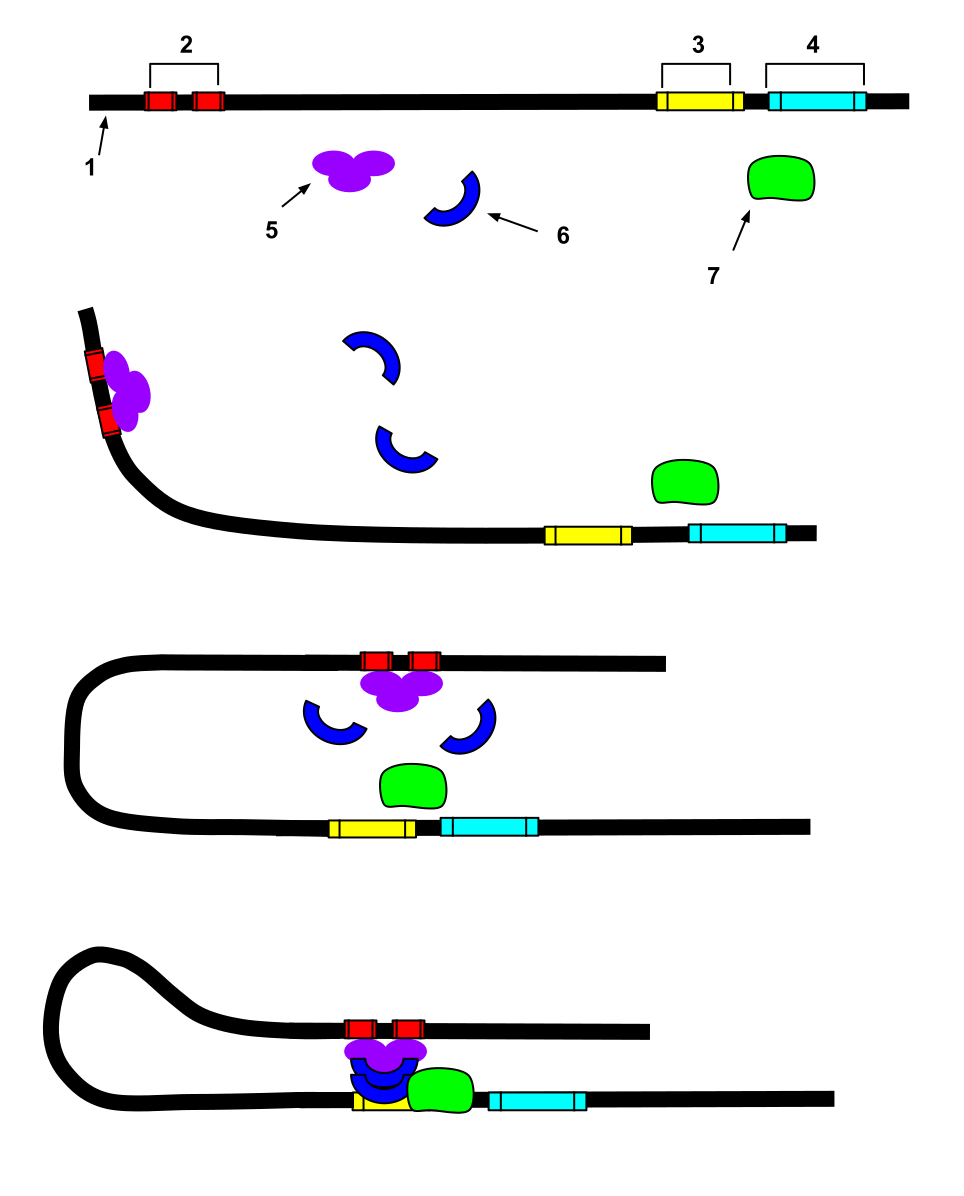
\includegraphics[scale=0.33, trim=0 650 0 0, clip]{Enhancer_Nucleotide_Sequence}}
    \only<2->{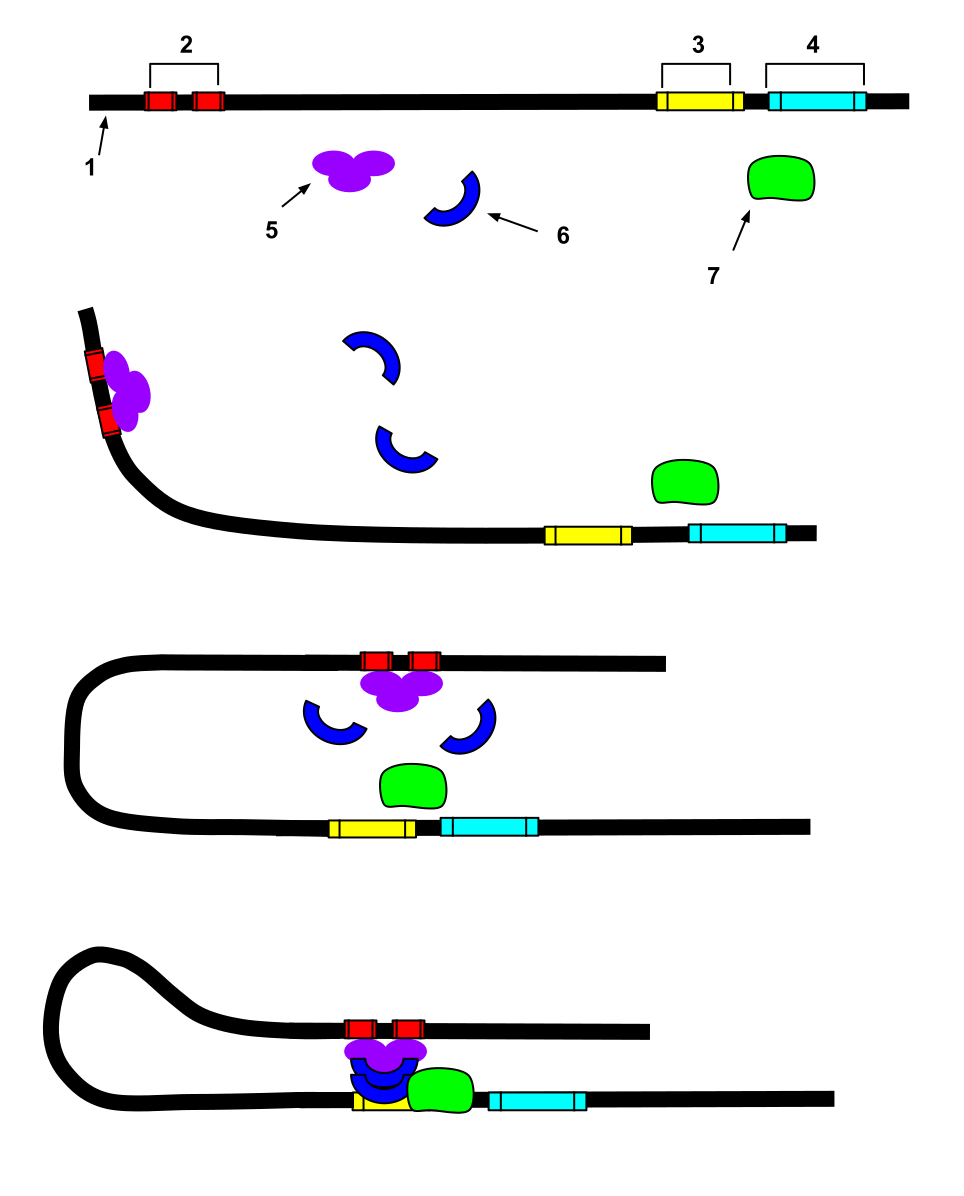
\includegraphics[scale=0.33, trim=0 70 0 580, clip]{Enhancer_Nucleotide_Sequence}}
    Image adapted from \cite{figenhancers}.

    % Explain workings of enhancers and promoters in short
    % it is relevant for them to have spatial proximity
    % 
\end{frame}

% Inhalt Vortrag:
% - Kurze motivation was man da machen will
% - Hi-C, grobe Erklärung was da passiert
% - Algorithmus selbst im Detail
% - Implementation ein paar erkenntnisse / schmankerl
% - Resultate
